\documentclass[11pt]{article}

\usepackage[margin=1in]{geometry}
\usepackage{hyperref}
\usepackage{tikz}
\usepackage{booktabs}
\usepackage{enumitem}
\usepackage{xcolor}
\usepackage{listings}
\usepackage{parskip}
\usepackage{amssymb}
\usetikzlibrary{positioning, arrows.meta, shapes.geometric, fit, backgrounds}

\hypersetup{
  colorlinks=true,
  linkcolor=black,
  urlcolor=blue!60!black,
  citecolor=black
}

\lstdefinelanguage{tsx}{
  keywords={import, export, from, async, await, function, return, const, let, default, new, if, else, true, false},
  keywordstyle=\color{blue!70!black}\bfseries,
  ndkeywords={Suspense, Home, BoardData, BoardSkeleton, OrdersBoard, findAllOrders, Promise, React},
  ndkeywordstyle=\color{purple!70!black}\bfseries,
  sensitive=true,
  comment=[l]{//},
  commentstyle=\color{gray!70!black}\itshape,
  string=[b]',
  stringstyle=\color{green!40!black},
  morestring=[b]"
}

\lstset{
  basicstyle=\ttfamily\footnotesize,
  frame=single,
  framesep=4pt,
  breaklines=true,
  columns=fullflexible,
  keepspaces=true,
  showstringspaces=false,
  language=tsx
}

\title{\textbf{Progressive Initial Load for Polaris}\\\large Shell First, Data After, with Room to Nest}
\author{Ahmed Khan}
\date{\today}

\begin{document}
\maketitle

\begin{abstract}
\noindent The Polaris home page currently blocks on a single database query before emitting any HTML, so first paint waits for \texttt{findAllOrders()} and the user sees a blank viewport during that round-trip. This document describes the minimum structural change that turns first paint into a shell-first, streamed render: a synchronous \texttt{Home} component, a \texttt{<Suspense>} boundary with a layout-accurate skeleton, and an async \texttt{BoardData} child that awaits the database and flushes real tiles when ready. The pattern is the same one Meta, Vercel, and Shopify ship in production, and it is designed to nest: when order tiles later acquire sub-objects (SKUs, quantities, customer details), each new data layer becomes another \texttt{<Suspense>} with its own skeleton.
\end{abstract}

\section{The Lag}

Before this change, \texttt{app/page.tsx} was a single \texttt{async} server component:

\begin{lstlisting}
export default async function Home() {
  const initial = await findAllOrders()
  return <OrdersBoard initial={initial} />
}
\end{lstlisting}

The render pipeline this produces:

\begin{enumerate}[leftmargin=1.4em, itemsep=0.15em]
  \item Browser requests \texttt{/}.
  \item Next.js invokes \texttt{Home()}. The \texttt{await} parks rendering.
  \item Postgres executes \texttt{SELECT * FROM orders}.
  \item The query resolves; \texttt{Home()} returns \texttt{<OrdersBoard>}.
  \item Next.js serialises the RSC payload and streams HTML.
  \item Browser paints. First meaningful paint has now cost one full DB round-trip plus serialisation.
\end{enumerate}

The blank screen during step 3 is the visible problem. Even with fast queries (sub-50\,ms on an empty table), first paint is gated on the slowest data dependency in the component. The lag only gets worse as the dataset grows, as the schema grows joins, or as the operator's network degrades.

\section{The Principle: Layered Rendering}

The production-grade fix is not ``make the query faster'' but ``don't block the shell on the query at all.'' Render what we already know --- the page chrome, the column layout, a visual anchor for where tiles will appear --- before we know anything about the data. Let the data arrive into the anchor over the same HTTP response, streamed in a later chunk.

Three conceptual layers, each with its own paint budget:

\begin{center}
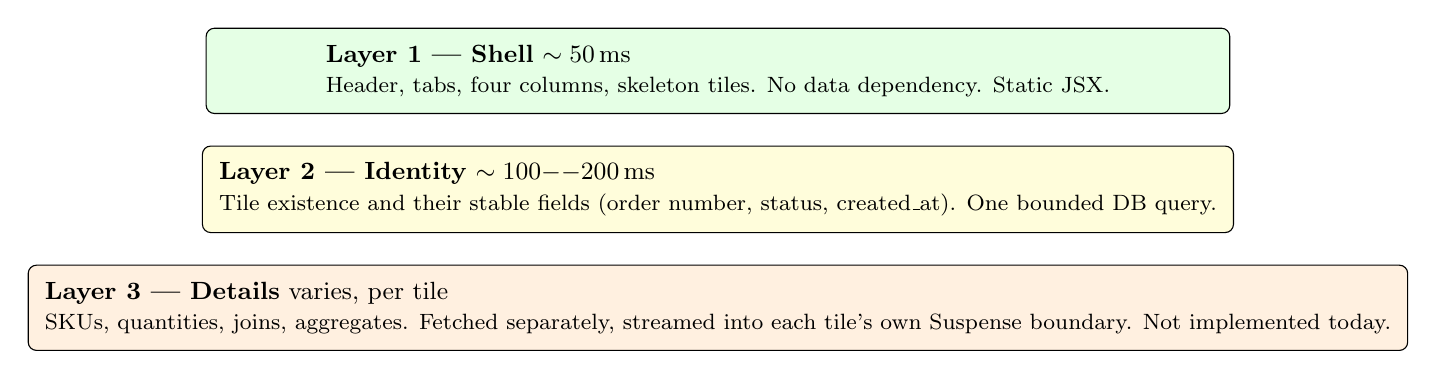
\begin{tikzpicture}[
  node distance=0.4cm,
  layer/.style={draw, rounded corners=3pt, minimum width=13cm, minimum height=1.0cm, align=left, font=\small, inner sep=6pt},
  shell/.style={layer, fill=green!10},
  identity/.style={layer, fill=yellow!14},
  details/.style={layer, fill=orange!12}
]
  \node[shell] (l1) {\textbf{Layer 1 --- Shell} \hfill $\sim 50$\,ms \\
    \footnotesize Header, tabs, four columns, skeleton tiles. No data dependency. Static JSX.};
  \node[identity, below=of l1] (l2) {\textbf{Layer 2 --- Identity} \hfill $\sim 100\text{--}200$\,ms \\
    \footnotesize Tile existence and their stable fields (order number, status, created\_at). One bounded DB query.};
  \node[details, below=of l2] (l3) {\textbf{Layer 3 --- Details} \hfill varies, per tile \\
    \footnotesize SKUs, quantities, joins, aggregates. Fetched separately, streamed into each tile's own Suspense boundary. Not implemented today.};
\end{tikzpicture}
\end{center}

Each layer lives behind a \texttt{<Suspense>} boundary. React's streaming renderer walks the tree; when it hits an unresolved promise it emits the fallback into the current HTML chunk and registers a continuation. The server continues resolving the rest of the tree in parallel and flushes additional chunks as each boundary settles. The browser paints each chunk as it arrives.

The change described here installs layer 1 and layer 2 today. Layer 3 is a forward-compatible extension that drops in when tiles gain sub-objects --- no rewrite of layers 1 or 2 required.

\section{The Implementation}

Two files, roughly forty lines total.

\subsection{\texttt{app/page.tsx} --- synchronous shell + async data}

\begin{lstlisting}
import { Suspense } from 'react'
import { findAllOrders } from '@/lib/db/orderRepository'
import { BoardSkeleton } from './BoardSkeleton'
import { OrdersBoard } from './OrdersBoard'

export default function Home() {
  return (
    <Suspense fallback={<BoardSkeleton />}>
      <BoardData />
    </Suspense>
  )
}

async function BoardData() {
  const initial = await findAllOrders()
  return <OrdersBoard initial={initial} />
}
\end{lstlisting}

\texttt{Home} is now synchronous. It returns immediately with a tree that React can begin emitting to the client on the first chunk. \texttt{BoardData} is the async boundary; its \texttt{await} no longer gates the response --- it only gates the resolution of its own \texttt{<Suspense>}.

\subsection{\texttt{app/BoardSkeleton.tsx} --- a layout-accurate placeholder}

The skeleton's job is to claim the same pixels the real board will occupy, so the transition from fallback to content causes \emph{no layout shift}. It copies the main element's flex chain, the horizontal column scroller, and the column dimensions verbatim, then fills each column with a fixed number of \texttt{animate-pulse} tile-shaped rectangles.

\begin{lstlisting}
const COLUMNS = ['Drafting', 'Reviewing', 'Invoicing', 'Archiving'] as const
const SKELETON_TILES_PER_COLUMN = 4

export function BoardSkeleton() {
  return (
    <main className="flex min-h-0 flex-1 flex-col gap-6 overflow-hidden p-6">
      <header className="shrink-0 flex items-center justify-between">
        <h1 className="text-xl font-semibold text-zinc-50">Orders</h1>
        <div aria-hidden className="h-8 w-[86px] rounded-md bg-zinc-800 animate-pulse" />
      </header>
      <div className="flex-1 min-h-0 flex overflow-x-auto scrollbar-thin pb-2">
        <div className="flex gap-4 pr-4">
          {COLUMNS.map((column) => (
            <section key={column} className="flex w-64 shrink-0 min-h-0 flex-col gap-3 rounded-lg border border-zinc-800 bg-zinc-900 p-3">
              { /* column header + 4 pulsing tile rectangles */ }
            </section>
          ))}
        </div>
      </div>
    </main>
  )
}
\end{lstlisting}

A few design choices worth calling out explicitly:

\begin{itemize}[leftmargin=1.4em, itemsep=0.15em]
  \item \textbf{Same \texttt{<main>} classes.} The skeleton's outer container matches the real board byte-for-byte. If the flex chain changes in \texttt{OrdersBoard.tsx}, the skeleton has to change with it. The close coupling is a feature, not a bug --- it guarantees the anchor doesn't lie about where content is about to appear.
  \item \textbf{Same column widths (\texttt{w-64}).} Horizontal scroll position is preserved through the transition.
  \item \textbf{Four columns always.} Every column renders a skeleton regardless of today's ``only Drafting has data'' behaviour, because tomorrow any column may. Bias the placeholder toward the final state, not the current state.
  \item \textbf{Tile-shaped rectangles} (\texttt{h-8}, \texttt{rounded-md}, \texttt{border border-zinc-700}, \texttt{bg-zinc-800}). Real tiles share the exact same classes, so the swap looks like content materialising rather than a different component mounting.
  \item \texttt{animate-pulse} from Tailwind. No library. No CSS written.
  \item \texttt{aria-hidden} on every purely-decorative skeleton node. Screen readers should not announce ``four pulsing regions''; they should announce ``Orders loading'' via the live region that the real board installs on arrival.
\end{itemize}

\section{Rendering Pipeline, Under the Hood}

The difference at the wire level is the shape of the HTTP response. Before:

\begin{center}
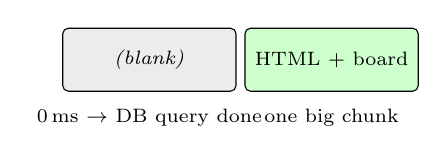
\begin{tikzpicture}[
  node distance=0.1cm,
  chunk/.style={draw, rounded corners=2pt, minimum width=2.2cm, minimum height=0.8cm, align=center, font=\scriptsize}
]
  \node[chunk, fill=gray!15] (wait) {\textit{(blank)}};
  \node[chunk, fill=green!20, right=of wait] (html) {HTML + board};
  \node[below=0.1cm of wait, font=\scriptsize] {$0$\,ms $\to$ DB query done};
  \node[below=0.1cm of html, font=\scriptsize] {one big chunk};
\end{tikzpicture}
\end{center}

After:

\begin{center}
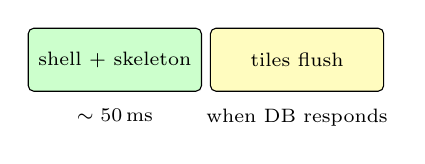
\begin{tikzpicture}[
  node distance=0.1cm,
  chunk/.style={draw, rounded corners=2pt, minimum width=2.2cm, minimum height=0.8cm, align=center, font=\scriptsize}
]
  \node[chunk, fill=green!20] (shell) {shell + skeleton};
  \node[chunk, fill=yellow!25, right=of shell] (board) {tiles flush};
  \node[below=0.1cm of shell, font=\scriptsize] {$\sim 50$\,ms};
  \node[below=0.1cm of board, font=\scriptsize] {when DB responds};
\end{tikzpicture}
\end{center}

React's server renderer walks the tree depth-first. When it encounters \texttt{<BoardData>}, \texttt{BoardData} returns a promise (because it is an async function). React ``suspends'' that subtree, records the fallback (\texttt{<BoardSkeleton />}), and continues rendering siblings. As soon as the rendered prefix has a complete set of non-suspended nodes, Next.js flushes the first HTTP chunk containing the shell and the skeleton, and the browser paints. In parallel, the server is still awaiting the \texttt{findAllOrders()} promise. When that resolves, React renders the suspended subtree and Next.js flushes a second chunk --- an HTML \texttt{<template>} plus a few bytes of RSC protocol instructing the client runtime to replace the skeleton node with the real tile content. The client reconciles without a full re-render.

The entire transition happens over a single HTTP response using chunked transfer encoding. There is no second round-trip, no client-side fetch, and no hydration delay beyond what would have existed anyway.

\section{Interaction with Realtime and Optimistic State}

\texttt{OrdersBoard} is a client component. It owns \texttt{useState}, \texttt{useOptimistic}, and the Supabase Realtime subscription set up in \texttt{useEffect}. None of that changes.

The flow is unchanged from the client's point of view: once the real \texttt{<OrdersBoard>} flushes into the DOM, it mounts, runs its \texttt{useEffect}, opens the Realtime channel, and begins accepting \texttt{INSERT}\,/\,\texttt{UPDATE}\,/\,\texttt{DELETE} events. Optimistic inserts via \texttt{addOptimistic} continue to prepend tiles in place. The skeleton never mounts as a React component on the client --- it is pure server-rendered HTML that React's reconciler replaces when the suspended subtree resolves. There is no coordination overhead between the skeleton and the live board.

This is why the change is so cheap: it is a pure server-render restructuring. The client-side concerns (subscriptions, optimistic state, mutations) live entirely below the Suspense boundary and are not aware that any boundary exists above them.

\section{Extending to Sub-Objects}

The same principle nests. When order tiles later gain sub-objects --- SKU lines, quantities, customer metadata --- each tile grows its own internal Suspense boundary:

\begin{lstlisting}
function Tile({ order, detailsPromise }) {
  return (
    <div className="...tile classes...">
      <header>#{order.orderNumber}</header>
      <Suspense fallback={<SkuListSkeleton />}>
        <TileDetails promise={detailsPromise} />
      </Suspense>
    </div>
  )
}
\end{lstlisting}

The parent server component (\texttt{BoardData}) fires the identity query as today, then kicks off a batched \texttt{findOrderDetailsMany(ids)} \emph{without} awaiting, and passes the raw promise through to each tile. The client unwraps with \texttt{use()}; React's Suspense boundary handles the fallback until the promise settles. A single batched query avoids N+1 at the database; per-tile Suspense gives the user ``tile numbers now, tile contents as they arrive'' visually.

Critically, nothing in layers 1 or 2 changes when layer 3 ships. The shell remains synchronous. Identity still resolves via the same query. Only the tile renderer gains a nested boundary. This is the shape of the pattern at every depth: each data layer is a self-contained Suspense boundary with its own skeleton and its own resolution timeline.

\section{What This Change Is Not}

Worth naming so scope does not drift:

\begin{itemize}[leftmargin=1.4em, itemsep=0.15em]
  \item \textbf{Not pagination.} The query is still \texttt{findAllOrders}. Bounding the kanban to a recent window is a separate concern documented elsewhere.
  \item \textbf{Not caching.} \texttt{unstable\_cache} around \texttt{findAllOrders} would make the DB round-trip disappear for repeat visits, but it is orthogonal to the streaming shape and can layer on top later.
  \item \textbf{Not Partial Prerendering.} PPR (Next.js 16's build-time pre-render of the static shell) would move shell paint from $\sim 50$\,ms to $\sim 0$\,ms by serving it from the CDN. It is a further optimisation on top of what this change delivers and is an opt-in per-route configuration.
  \item \textbf{Not a route \texttt{loading.tsx}.} A \texttt{loading.tsx} file would provide the same skeleton for \emph{navigations} to \texttt{/}. This change handles the initial render. Both can coexist; \texttt{loading.tsx} is a future add.
\end{itemize}

\section{Trade-offs and Non-Obvious Properties}

\begin{itemize}[leftmargin=1.4em, itemsep=0.15em]
  \item \textbf{The skeleton must track the real layout.} If \texttt{OrdersBoard}'s outer flex chain or column width changes and the skeleton does not, first paint shifts when real content arrives --- the exact bug the skeleton exists to prevent. Treat the two files as a visual pair; diff them together.
  \item \textbf{Streaming degrades to batch when hosts buffer.} Reverse proxies and some edge runtimes coalesce chunks. If the deployment target silently buffers the response, streaming collapses back to a single-chunk paint --- the user experience becomes no worse than today, just no better. Next.js on Node on Vercel supports end-to-end chunked transfer; Cloudflare Workers, Fly.io, and self-hosted setups behind nginx with default buffering may require configuration.
  \item \textbf{RSC payload size grows slightly.} The skeleton JSX is sent alongside the real content (the client runtime needs to know how to reconcile). For a skeleton this small it is irrelevant, but do not stuff a 200-node ornate skeleton into the fallback --- its bytes are on the critical path.
  \item \textbf{Fallback-to-content flash.} If the DB query is fast enough that the query resolves before the shell is painted, the client still briefly renders the skeleton and then replaces it. React 19's transitions can suppress this flash for later navigations; for initial loads, a sub-50\,ms skeleton flash is acceptable and expected.
  \item \textbf{No changes to Realtime wiring.} Supabase channels, validation, optimistic inserts, and the \texttt{New Order} server action all work exactly as before. This change lives entirely in the server-render layer.
\end{itemize}

\section{Verification}

Manual, in the browser:

\begin{enumerate}[leftmargin=1.4em, itemsep=0.15em]
  \item \texttt{npm run dev}.
  \item Open \texttt{/} with DevTools $\to$ Network throttling set to \emph{Slow 3G}. Without this change, the viewport stays blank until the entire response arrives. With this change, the shell and four pulsing columns appear in the first chunk; the tile content fills in when \texttt{findAllOrders()} resolves.
  \item Observe the HTML stream in the Network panel: the initial response body is split across multiple chunks, and the second chunk contains a \texttt{<template>} element whose markup replaces the skeleton placeholder via the RSC runtime.
  \item Create an order: the optimistic tile still appears instantly; the Realtime channel still reconciles it; nothing in the interactive path changed.
  \item Check that layout is stable --- no visible shift when tiles replace the skeleton. If there is a shift, the skeleton's dimensions are out of sync with the real tile dimensions and need to be reconciled.
\end{enumerate}

Automated: no new tests. The change is a server-render restructuring with no new logic to cover; the existing suite continues to exercise \texttt{findAllOrders} and the \texttt{OrdersBoard} interaction paths.

\section{File Inventory}

\begin{table}[h]
  \centering
  \begin{tabular}{@{}llp{7.5cm}@{}}
    \toprule
    File & Status & Role \\
    \midrule
    \texttt{app/page.tsx} & modified & Now synchronous; wraps data fetch in \texttt{<Suspense>}. \\
    \texttt{app/BoardSkeleton.tsx} & new & Layout-accurate placeholder for the fallback slot. \\
    \texttt{app/OrdersBoard.tsx} & unchanged & Receives \texttt{initial} prop as before. \\
    \texttt{lib/db/orderRepository.ts} & unchanged & \texttt{findAllOrders} untouched. \\
    \bottomrule
  \end{tabular}
\end{table}

\noindent Two files touched. Forty lines of real change. First paint decoupled from the database.

\end{document}
